\documentclass[tikz]{standalone}
\usepackage{xcolor}
\definecolor{bg}{HTML}{171D2B}
\definecolor{aksen}{HTML}{F7B538}
\begin{document}
\pagecolor{bg}
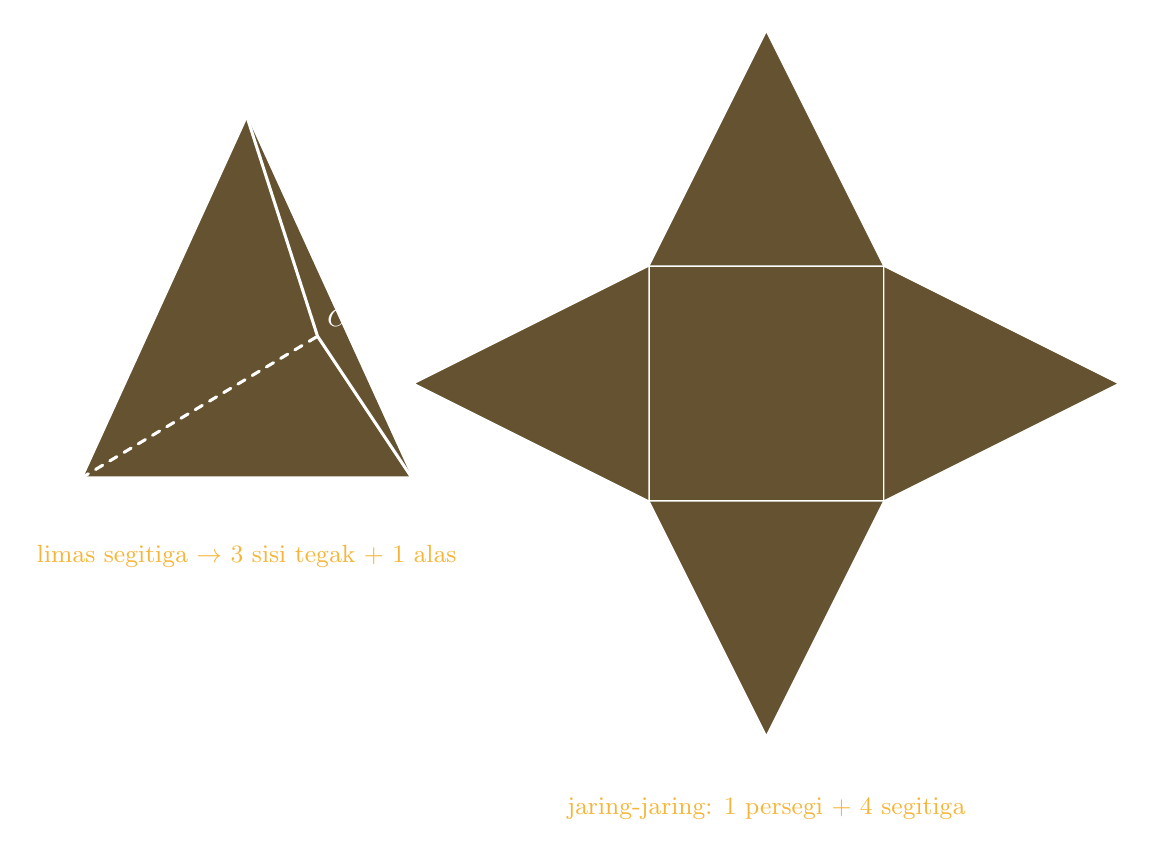
\begin{tikzpicture}[
  line cap=round, line join=round,
  x=1cm, y=1cm,
  warnai/.style={draw=white, line width=1.1pt, fill=aksen!35!bg},
  label/.style={text=white, font=\small},
  ukur/.style={text=aksen, font=\small},
]
  % ===== KIRI: LIMAS SEGITIGA (TETRAHEDRON) =====
  \begin{scope}[shift={(0,0)}]
    % titik puncak dan alas segitiga
    \coordinate (P) at (0,3.4);
    \coordinate (A) at (-2.1,-1.2);
    \coordinate (B) at (2.1,-1.2);
    \coordinate (C) at (0.9,0.6);
    \draw[warnai] (P) -- (A) -- (B) -- cycle;
    \draw[warnai] (P) -- (C) -- (B);
    \draw[warnai, dashed, fill=none] (A) -- (C);
    \node[label] at (P) [above] {$P$};
    \node[label] at (A) [below left] {$A$};
    \node[label] at (B) [below right] {$B$};
    \node[label] at (C) [above right] {$C$};
    \node[label, text=aksen] at (0,-2.2) {limas segitiga $\to$ 3 sisi tegak + 1 alas};
  \end{scope}

  % ===== KANAN: JARING-JARING LIMAS SEGIEMPAT =====
  \begin{scope}[shift={(6.6,0)}]
    % alas persegi 3x3, puncak jaring di tengah sisi atas
    \coordinate (K1) at (-1.5,-1.5);
    \coordinate (K2) at ( 1.5,-1.5);
    \coordinate (K3) at ( 1.5, 1.5);
    \coordinate (K4) at (-1.5, 1.5);
    % sisi tegak atas: segitiga duduk di sisi K3-K4, tinggi 3
    \coordinate (P) at (0, 4.5);
    % sisi tegak kanan: duduk di K2-K3, tinggi 3 ke kanan
    \coordinate (Q) at (4.5, 0);
    % sisi tegak bawah
    \coordinate (R) at (0, -4.5);
    % sisi tegak kiri
    \coordinate (S) at (-4.5, 0);
    \draw[warnai] (K1) -- (K2) -- (K3) -- (K4) -- cycle;
    \draw[warnai] (K4) -- (P) -- (K3);
    \draw[warnai] (K3) -- (Q) -- (K2);
    \draw[warnai] (K2) -- (R) -- (K1);
    \draw[warnai] (K1) -- (S) -- (K4);
    \node[label, text=aksen] at (0,-5.4) {jaring-jaring: 1 persegi + 4 segitiga};
  \end{scope}
\end{tikzpicture}
\end{document}
